\documentclass[11pt,a4paper,titlepage]{article}
\usepackage{amsmath}
\usepackage{amssymb}
\usepackage{wasysym}
\usepackage{float}
\usepackage{latexsym,amsmath,amssymb}
\usepackage{graphicx}
\usepackage{epstopdf}
%\usepackage{subfig}
\usepackage{slashed}
\usepackage{bm}
\usepackage{epsfig}
\usepackage{cases}
\usepackage{dcolumn}
\usepackage{color}
\usepackage[colorlinks=true,linkcolor=red]{hyperref}
\usepackage{listings} 
\usepackage{xcolor} % for setting colors
\begin{document}
\begin{titlepage}
%\vspace*{3cm}
\begin{center}
\Huge {A tutorial on GiNaCDE-GUI to solve Differential Equations} 
\end{center}
\vspace{3cm}
\begin{center}
\Large{GiNaCDE-GUI (V1.5.0)}
\end{center}
\vspace{2cm} 
\begin{center} 
Mithun Bairagi \\[3pt]  
\textit{Department of Physics, The University of Burdwan, Golapbag 713104, West Bengal, India} \\ [1cm]
%\textit{Address} \\ [1cm] 
\today
\end{center}
\end{titlepage}
 
\clearpage
The usage of GiNaCDE-GUI for solving differential equations is described in this tutorial. The following two examples demonstrate the usage of GiNaCDE-GUI to solve differential equations.
\section{Example 1}
Let us consider the Eckhaus equation 
\begin{equation}\label{eckhaus}
	i{u_t} + {u_{xx}} + 2{\left( {{{\left| u \right|}^2}} \right)_x}u + {\left| u \right|^4}u = 0.
\end{equation}
For solving Eq. \eqref{eckhaus} using GiNaCDE library, the C++ codes are\\
\begin{verbatim}
	// eckhaus_FIM.cpp
	#include <GiNaCDE/GiNaCDE.h>
	int main()
	{
		   const ex u=reader("u"), t=reader("t"), x=reader("x"), 
		            a=reader("a"), b=reader("b"),k=reader("k");   
		   depend(u, {t, x});
		   const ex pde = I*Diff(u,t,1) + Diff(u,x,2) + 2*u*Diff(u*conjugate(u),x,1)
		                  + u*u*conjugate(u)*conjugate(u)*u;
		   output = mathematica;  
		   twcPhase=lst{lst{-2*k*a,k},lst{b,a}};
		   paraInDiffSolve=lst{};
		   filename = "eckhaus_FIM.txt";
		   desolve(pde,{u},FIM);
		   return 0;
	}
\end{verbatim}
In the following, we display the screenshots of each step when we implement the above C++ code in GiNaCDE-GUI.

\begin{figure}[H]
	\centering
	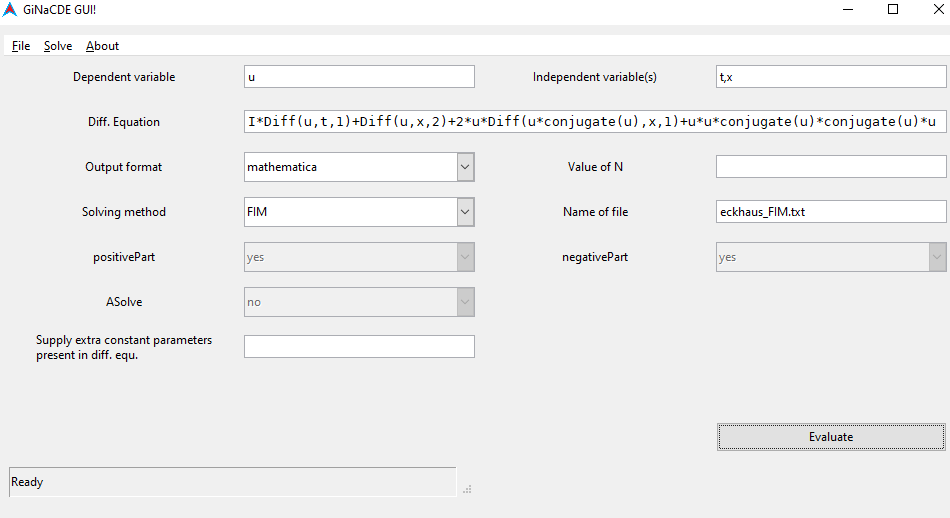
\includegraphics[width=\linewidth]{Ex1step1}
	\caption{ Step 1. }
	\label{fig:Ex1step1}
\end{figure}

\begin{figure}[H]
	\centering
	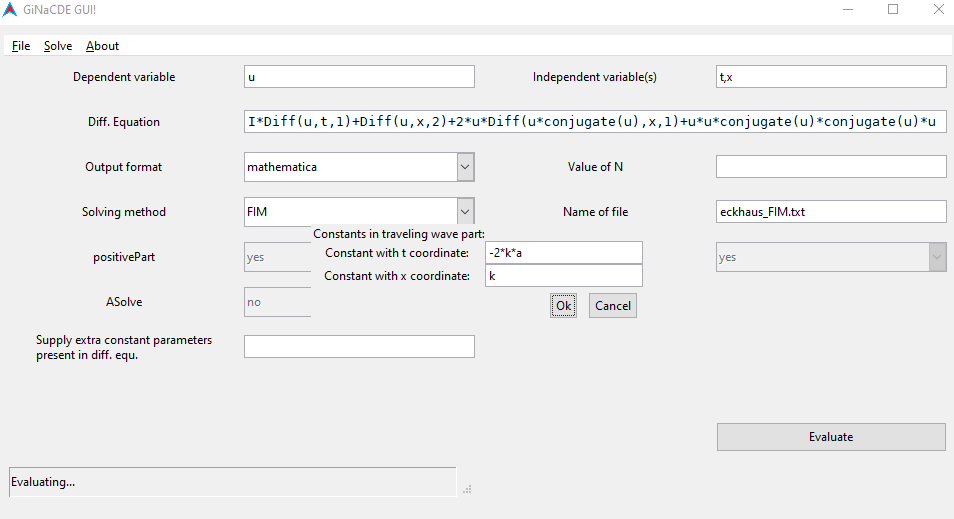
\includegraphics[width=\linewidth]{Ex1step2}
	\caption{ Step 2. }
	\label{fig:Ex1step2}
\end{figure}

\begin{figure}[H]
	\centering
	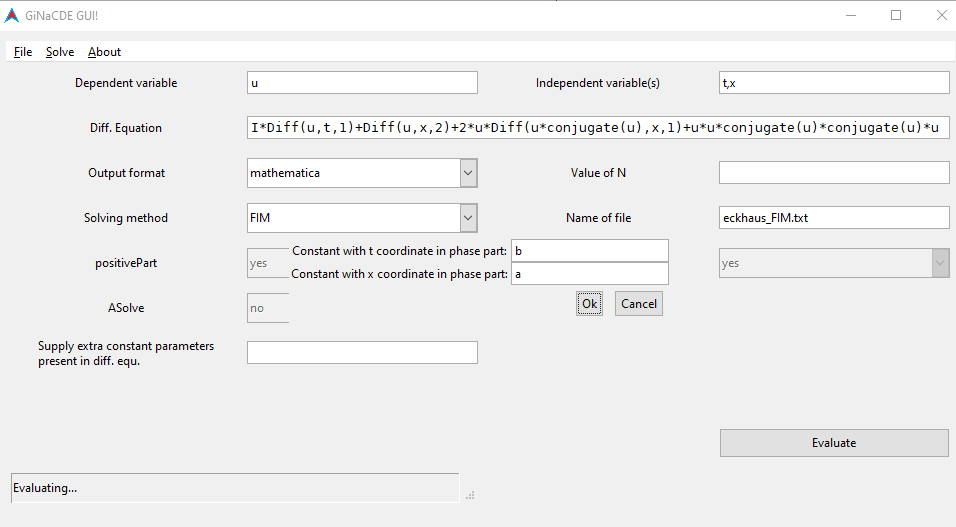
\includegraphics[width=\linewidth]{Ex1step3}
	\caption{ Step 3. }
	\label{fig:Ex1step3}
\end{figure}

\begin{figure}[H]
	\centering
	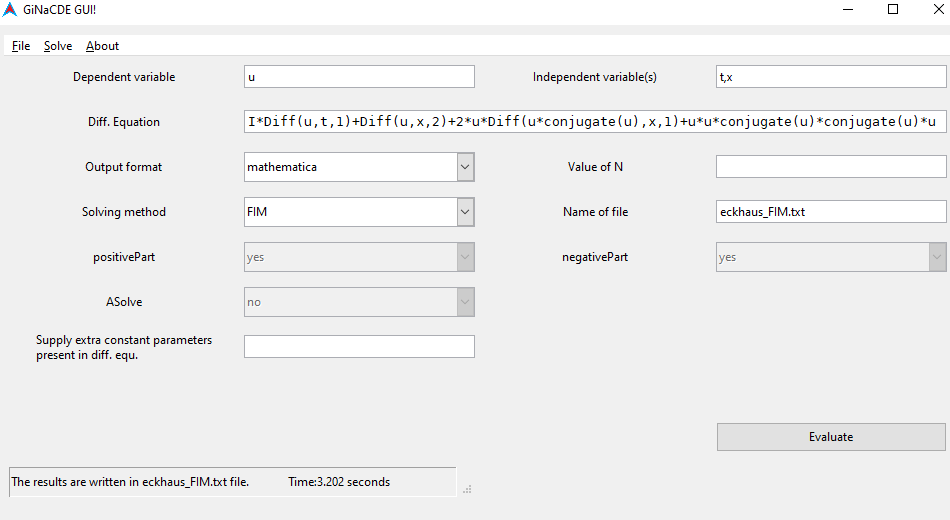
\includegraphics[width=\linewidth]{Ex1step4}
	\caption{ Step 4. }
	\label{fig:Ex1step4}
\end{figure}

After execution of the last step in fig. \ref{fig:Ex1step4} the output results are saved in \emph{eckhaus\_FIM.txt} file.
\section{Example 2}
We now discuss an another example considering generalized Camassa-Holm equation
\begin{equation}\label{Camassa}
	{u_t} + 2k{u_x} - {u_{xxt}} + au{u_x} - 2{u_x}{u_{xx}} - u{u_{xxx}} = 0.
\end{equation}
The following C++ code solve Eq. \eqref{Camassa} applying modified F-expansion method.
\begin{verbatim}
	// Generalized_Camassa-Holm_mF.cpp
	#include <GiNaCDE/GiNaCDE.h>
	int main()
	{
		   const ex u=reader("u"),t=reader("t"), x=reader("x"),
		            k=reader("k"),a=reader("a"),k_0=reader("k_0"),
		            k_1=reader("k_1"),A_1=reader("A_1"),A_3=reader("A_3");   
		   depend(u, {t,x});
		   const ex pde = Diff(u,t,1)+2*k*Diff(u,x,1)-Diff(Diff(u,x,2),t,1)
		                 +a*u*Diff(u,x,1)-2*Diff(u,x,1)*Diff(u,x,2)
		                 -u*Diff(u,x,3); 
		   output = maple;
		   twcPhase = lst{lst{k_0,k_1},lst{}};
		   degAcoeff = lst{3,0,A_1,0,A_3};
		   NValue = 2;
		   filename = "Generalized_Camassa-Holm_mF.txt";
		   ASolve=false;
		   positivePart = true; 
		   negativePart = true;
		   paraInDiffSolve = lst{k,a};
		   desolve(pde, {u}, mF_expansion);
		   return 0;
	}
\end{verbatim}
The following screenshots express each step to implement the above C++ code in GiNaCDE-GUI.


\begin{figure}[H]
	\centering
	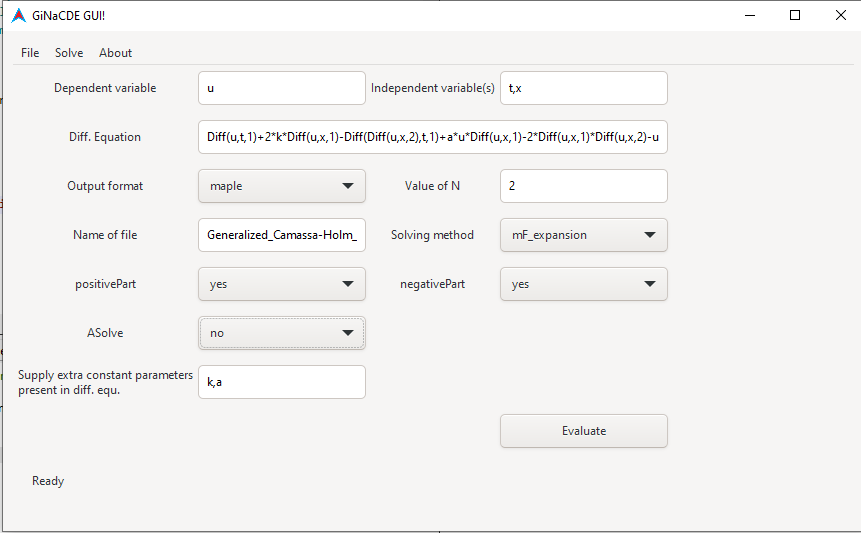
\includegraphics[width=\linewidth]{Ex2step1}
	\caption{ Step 1. }
	\label{fig:Ex2step1}
\end{figure}

\begin{figure}[H]
	\centering
	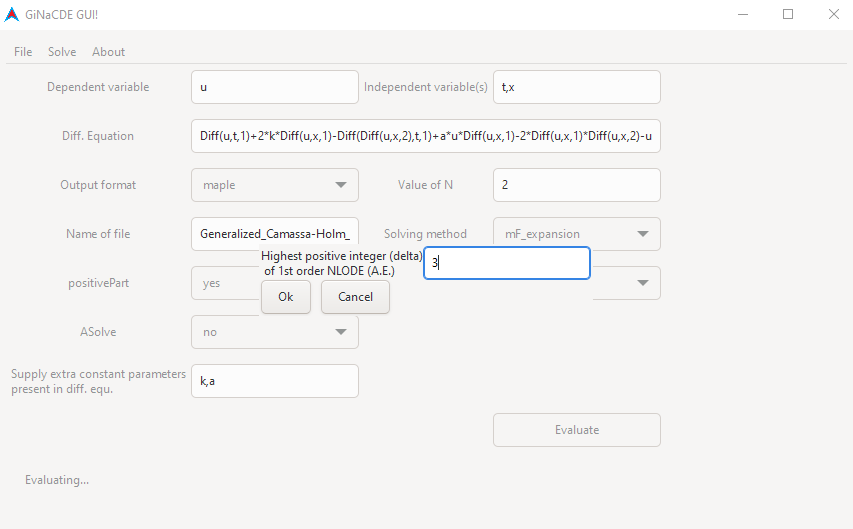
\includegraphics[width=\linewidth]{Ex2step2}
	\caption{ Step 2. }
	\label{fig:Ex2step2}
\end{figure}

\begin{figure}[H]
	\centering
	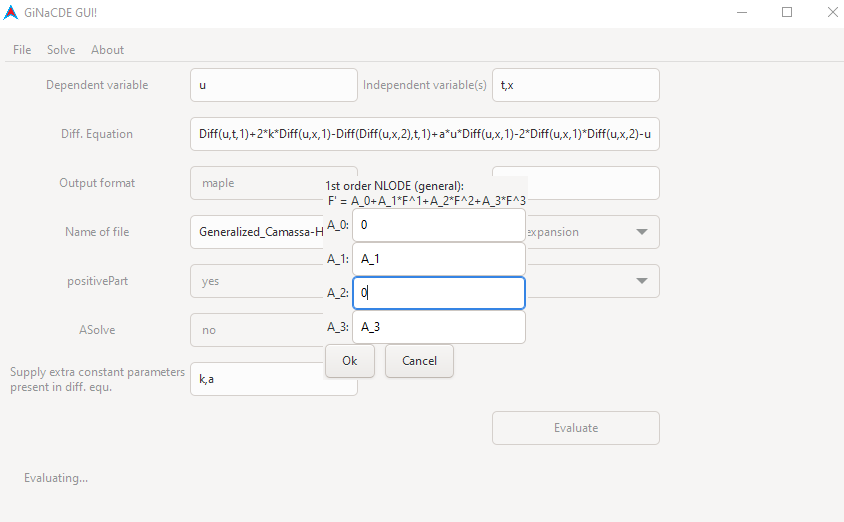
\includegraphics[width=\linewidth]{Ex2step3}
	\caption{ Step 3. }
	\label{fig:Ex2step3}
\end{figure}

\begin{figure}[H]
	\centering
	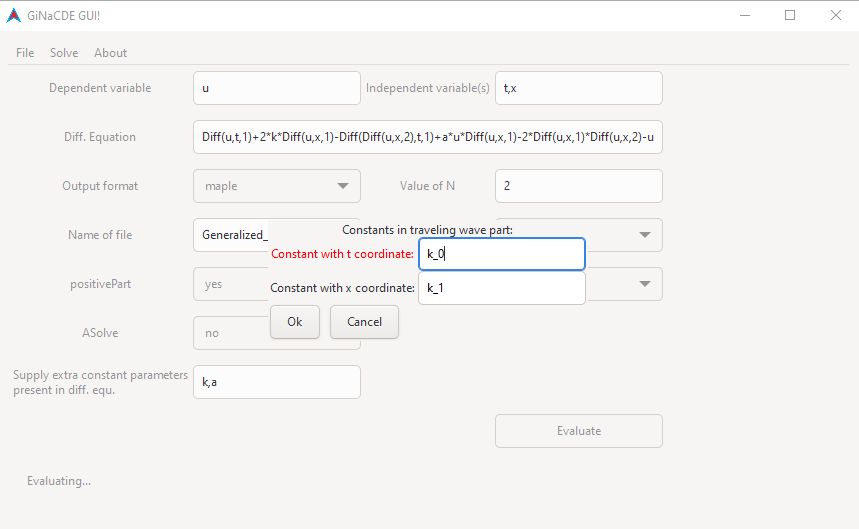
\includegraphics[width=\linewidth]{Ex2step4}
	\caption{ Step 4. }
	\label{fig:Ex2step4}
\end{figure}

\begin{figure}[H]
	\centering
	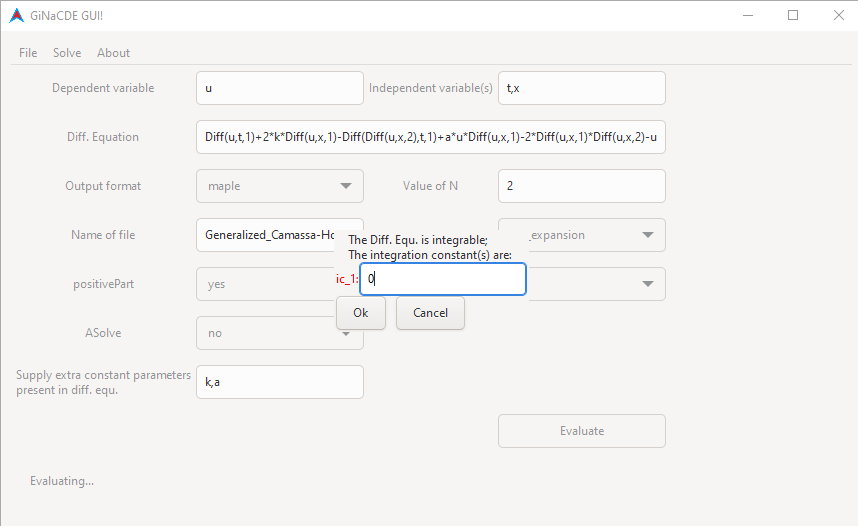
\includegraphics[width=\linewidth]{Ex2step5}
	\caption{ Step 5. }
	\label{fig:Ex2step5}
\end{figure}

\begin{figure}[H]
	\centering
	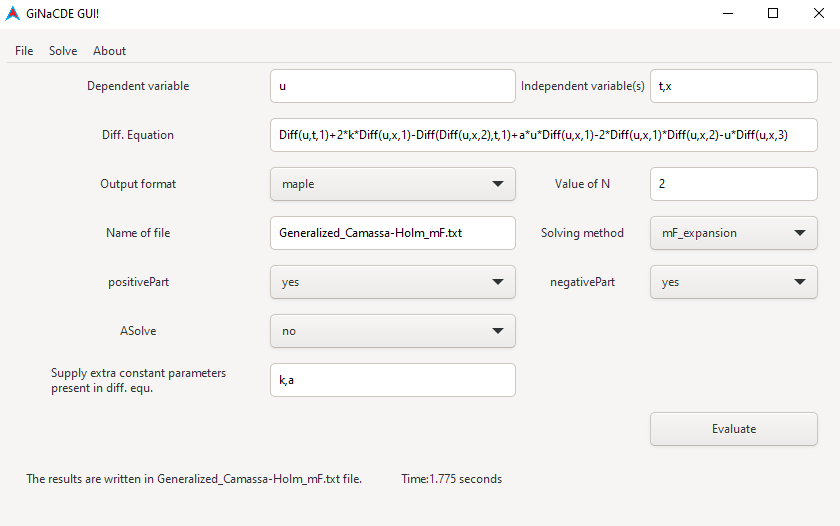
\includegraphics[width=\linewidth]{Ex2step6}
	\caption{ Step 6. }
	\label{fig:Ex2step6}
\end{figure}
After execution of the last step in fig. \ref{fig:Ex2step6} the output results are saved in \emph{Generalized\_Camassa-Holm.txt} file.
\end{document}